\documentclass[12pt]{article}

\usepackage[left=0.9in,right=0.9in,top=0.8in,bottom=1.05in]{geometry}
\newcommand{\ligne}[1]{\rule[0.5ex]{\textwidth}{#1}\\}

\usepackage[]{graphicx}
\usepackage{amsmath}
%\usepackage{wrapfig}
%\usepackage{physics}

\begin{document}

\noindent
Sean Gravelle\\
Numerical PDEs Homework \#2\\

% \noindent \textbf{For all problems asking for a graph:} you do not need to write up the method you programmed. Including plots of your solution and convergence is sufficient for full credit. The ideal homework will have one, information-dense and properly labeled figure with a caption and a \textit{brief} discussion. \textbf{You must type up your HW.} I don't care if it's word or Tex as long as it's well organized, easy to follow, and submitted as a pdf. 

\vspace{0.3cm}

\subsection*{Problem 1: Basic Poisson Equation}

Error plot for basic problem
\[\nabla^2u = f(x,y)\]

\begin{itemize}
\item
Domain: $x\in[0,2\pi]$ and $y\in[0,2\pi]$
\item
Right-hand side: $f(x,y) = -8\cos(2x)\sin(2y)$
\item
Dirichlet conditions on boundaries:
\begin{itemize}
\item
Top and bottom: $u(x,y)=0$
\item
Left and right: $u(x,y)=\sin(2y)$
\end{itemize}
\item
Test solution: $u(x,y) = \cos(2x)\sin(2y)$
\end{itemize}

\begin{center}
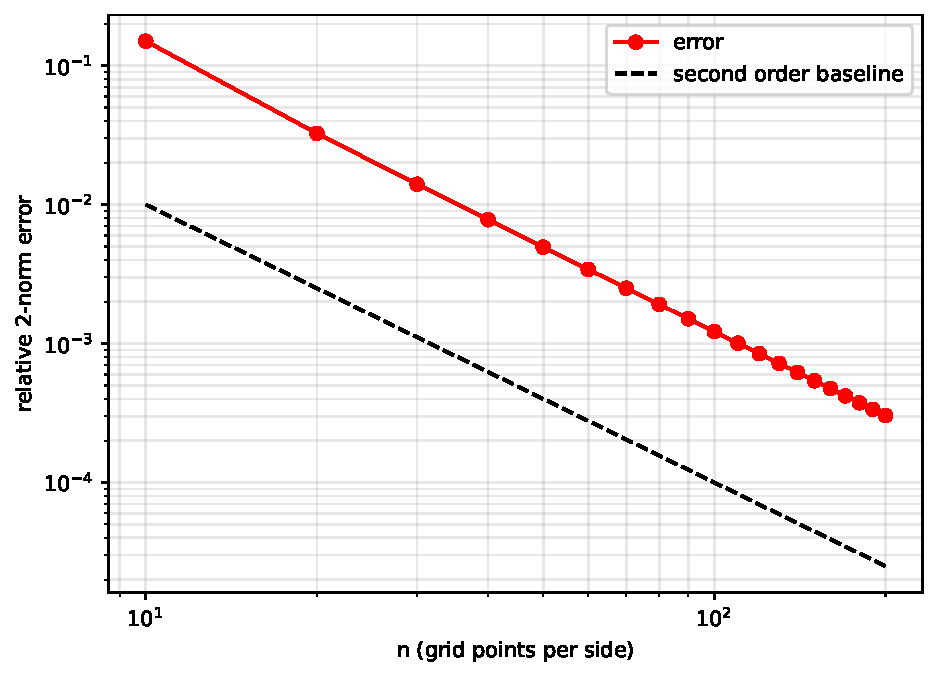
\includegraphics[width=\textwidth]{error_plot1.pdf}
\end{center}

\newpage
\subsection*{Problem 2: Poisson Equation with Immersed Boundary}

\begin{itemize}
\item
Immersed boundary points:
$x^{ib} = \pi + \cos(\theta)$,
$y^{ib} = \pi + \sin(\theta)$,
for $\theta\in[0,2\pi]$
\item
Dirichlet condition on immersed boundary:
$u(x^{ib},y^{ib}) = \cos(2x^{ib})\sin(2y^{ib})$
\end{itemize}

I solved this using GMRES with the following parameters:

\texttt{rtol = max(1e-12, 0.001*H*H)}

\texttt{restart = N*N*Nib}

\texttt{maxiter = 1}

Here, $N$ is the number of rectilinear gridpoints on each side, and $Nib$ is the number of immersed boundary points. In the immersed boundary grid, I chose $\Delta\theta=\Delta x$. I considered this a reasonable starting point because for small $\theta$, the small angle approximation gives $\sin(\theta)\approx\theta$, so the choice $\Delta\theta=\Delta x$ makes points on the circle separated by roughly the same distance as points on the rectilinear grid.

Error plot: $u$ is relative error as in problem 1; the ``error'' for $q$ is just the norm of $q$, since in this problem the correct charge is identically 0. While this method converges, we see from the plot below that convergence is at the slower rate of $1/N^{1.5}$, and the overall error is somewhat larger.

\begin{center}
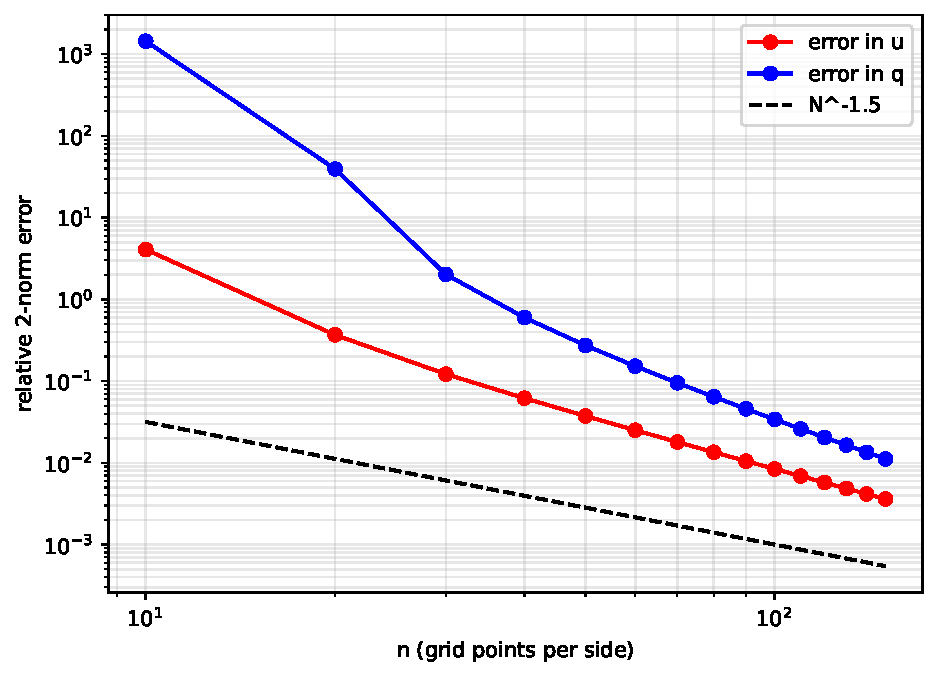
\includegraphics[width=\textwidth]{error_plot2.pdf}
\end{center}


\newpage
\subsection*{Problem 3}

Using the same code, I solved the same problem but with $f(x,y)=0$ and $u=0$ on all boundaries. The immersed boundary points, however, still satisfy the condition $u(x,y)=\cos(2x)\sin(2y)$, so the charges will be nonzero. The 3 dimensional plot is shown below.

\begin{center}
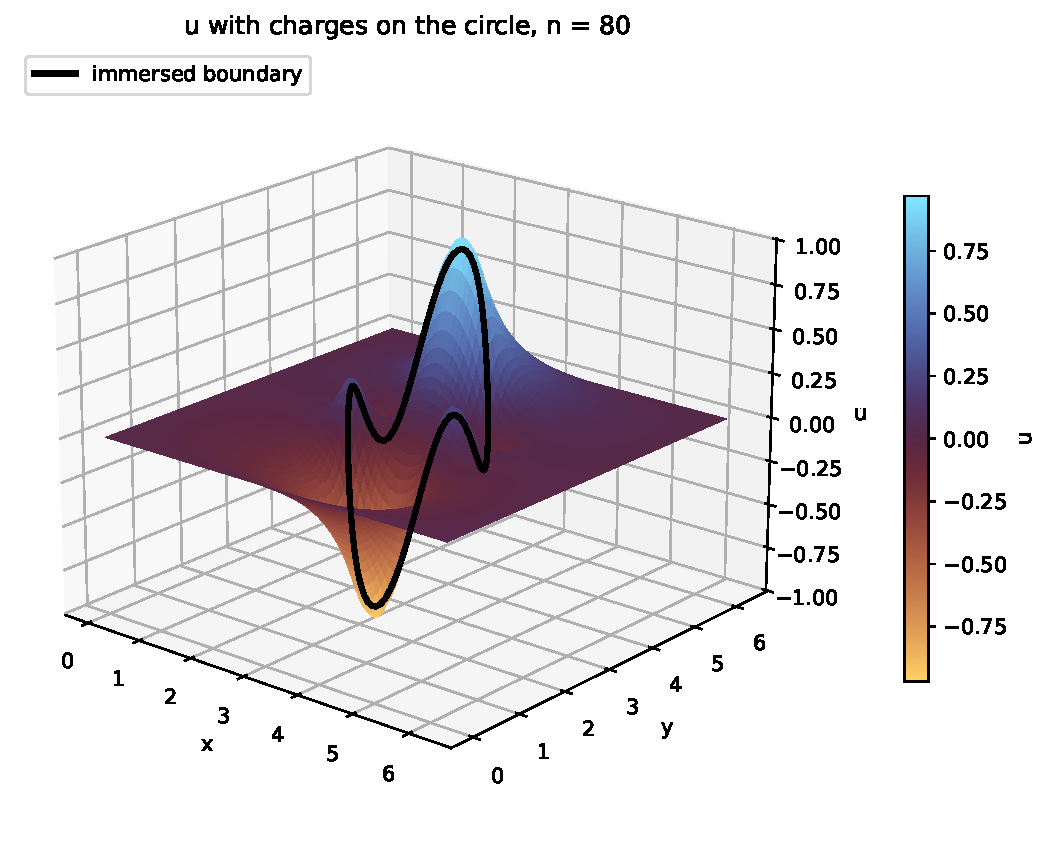
\includegraphics[width=\textwidth]{prob3plot.pdf}
\end{center}

\end{document}